%-------------------------------------------------------------------------------
%	EMPIEZA CAPITULO
%-------------------------------------------------------------------------------

\chapter{Diagramas de Bode}

    \begin{marginfigure}
        \centering
        \resizebox{\textwidth}{!}{
            \tikzstyle{block} = [draw, rectangle, minimum height=3em, minimum width=4em]

            \begin{tikzpicture}[auto, node distance=2cm, >=latex']
                \node [input, name=entrada] {};
                \node [block, right of=entrada] (planta) {$G(s)$};
                \node [output, right of=planta] (salida) {};

                \draw [->] (entrada) -- node[name=u] {$r(s)$} (planta);
                \draw [->] (planta) -- node[name=y] {$y(s)$} (salida);
            \end{tikzpicture}}
        \caption{\label{dia:bode1}Sistema Hurwitz estable.}
    \end{marginfigure}

    Dado el sistema de la figura~\ref{dia:bode1}, con $G(s)$ Hurwitz estable, sabemos que la ecuación del sistema será:

    \begin{equation*}
        y(s) = G(s) r(s)
    \end{equation*}

    asumimos que la entrada es de la forma:

    \begin{equation*}
        r(s) = X \left( \frac{\omega}{s^2 + \omega^2} \right)
    \end{equation*}

    y la planta es de la forma:

    \begin{equation*}
        G(s) = \frac{p(s)}{q(s)} = \frac{p(s)}{(s + s_1) (s + s_2) \dots (s + s_n)}
    \end{equation*}

    de donde se asumen polos simples de primero orden, aunque los reslutados por obtener se mantienen si los polos no lo son.

    Al sustituir pues en la ecuación del sistema, tendremos:

    \begin{eqnarray*}
        y(s) & = & X \left( \frac{\omega}{s^2 + \omega^2} \right) \frac{p(s)}{(s + s_1) (s + s_2) \dots (s + s_n)} \\
        & = & \frac{a}{s + j \omega} + \frac{\bar{a}}{s - j \omega} + \frac{b_1}{s + s_1} + \dots + \frac{b_n}{s + s_n}
    \end{eqnarray*}

    lo cual podemos resolver obteniendo la transformada inversa de Laplace:

    \begin{equation*}
        y(t) = a e^{-j \omega t} + \bar{a} e^{j \omega t} + b_1 e^{-s_1 t} + \dots + b_n e^{-s_n t}
    \end{equation*}

    lo cual implica que tendremos una salida en estado estacionario:

    \begin{equation*}
        y_{ss}(t) = \lim_{t \to \infty} y(t) = a e^{-j \omega t} + \bar{a} e ^{j \omega t}
    \end{equation*}

    es decir, cuando $t$ tiende a $\infty$ todos los polos del sistema se eliminan y nos queda el comportamiento de la entrada a seguir.

    Por otro lado, para obtener los valores de $a$ y $\bar{a}$ aplicamos fracciones parciales y obtenemos:

    \begin{eqnarray*}
        a & = & \left. G(s) X \left( \frac{\omega}{s^2 + \omega^2} \right) + (s + j \omega) \right|_{s=-j \omega} = - G(-j \omega) X \frac{1}{2j} \\
        \bar{a} & = & \left. G(s) X \left( \frac{\omega}{s^2 + \omega^2} \right) + (s - j \omega) \right|_{s=j \omega} = G(j \omega) X \frac{1}{2j}
    \end{eqnarray*}

    de donde sabemos que $G(j \omega)$ lo podemos escribir como su magnitud multiplicado por una exponencial de mangitud unitaria con el angulo deseado:

    \begin{eqnarray*}
        G(j \omega) & = & \left| G(j \omega) \right| e^{j \phi} \\
        G(-j \omega) & = & \left| G(j \omega) \right| e^{-j \phi}
    \end{eqnarray*}

    en donde $\phi = \phase{G(j \omega)} = \arctan{\left( \frac{\Im{G}}{\Re{G}} \right)}$.

    Por lo tanto, $a$ y $\bar{a}$ los podemos escribir como:

    \begin{eqnarray*}
        a & = & - \left| G(j \omega) \right| e^{-j \phi} X \frac{1}{2j} \\
        \bar{a} & = & \left| G(j \omega) \right| e^{j \phi} X \frac{1}{2j}
    \end{eqnarray*}

    Tomando esto en cuenta, la salida en estado estacionario nos quedará:

    \begin{eqnarray*}
        y_{ss}(t) & = & X \left| G(j \omega) \right| \frac{e^{j(\omega t + \phi)} - e^{-j(\omega t + \phi)}}{2j} \\
        & = & X \left| G(j \omega) \right| \sin{(\omega t + \phi)} \\
        & = & y \sin{(\omega t + \phi)}
    \end{eqnarray*}

    en donde $y = X \left| G(j \omega) \right|$ y $\phi = \phase{G(j \omega)}$.

%-------------------------------------------------------------------------------
%	EMPIEZA SECCION
%-------------------------------------------------------------------------------

    \newpage
    \section{Factores de primer orden}
        Para analizar ahora el comportamiento de una planta con factores de primer orden, proponemos el sistema siguiente:

        \begin{equation*}
            G(s) = \frac{1}{Ts + 1}
        \end{equation*}

        el cual tiene magnitud y fase:

        \begin{eqnarray*}
            \left| G(j \omega) \right| & = & \left| \frac{1}{j \omega T + 1} \right| = \frac{1}{\sqrt{1 + (\omega T)^2}} \\
            \left| G(j \omega) \right|_{dB} & = & 20 \log{\left| G(j \omega) \right|} = -20 \log{\sqrt{1 + (\omega T)^2}} \\
            \phi & = & - \arctan{(\omega T)}
        \end{eqnarray*}

        en donde a la magnitud le hemos sacado el $log_{10}$ y multiplicado por $20$ para expresarla en $dB$.

        De estas expresiones podemos ver, que para diferentes valores de $\omega T$ obtendremos diferentes valores de magnitud:

        \begin{eqnarray*}
            \omega T \ll 1 & \implies & \left| G(j \omega) \right|_{dB} \approx -20 \log{\sqrt{1}} = 0 dB \\
            \omega T \gg 1 & \implies & \left| G(j \omega) \right|_{dB} \approx -20 \log{\sqrt{(\omega T)^2}} = -20 \log{(\omega T)} dB \\
            \omega T = 1 & \implies & \left| G(j \omega) \right|_{dB} = -20 \log{\sqrt{2}} \approx -3 dB
        \end{eqnarray*}

        y de fase:

        \begin{eqnarray*}
            \omega T \ll 1 & \implies & -\arctan{(\omega T)} \approx - \arctan{(0)} = 0^o \\
            \omega T \gg 1 & \implies & -\arctan{(\omega T)} \approx - \arctan{(\infty)} = -90^o \\
            \omega T = 1 & \implies & -\arctan{(\omega T)} = - \arctan{(1)} = -45^o
        \end{eqnarray*}

        Con estas expresiones podemos trazar asintotas,  las cuales nos ayudarán a gráficar el diagrama de Bode del sistema $G(s) = \frac{1}{Ts + 1}$ en la figura~\ref{fig:bodeprimerorden}.

        \begin{marginfigure}
            \centering
            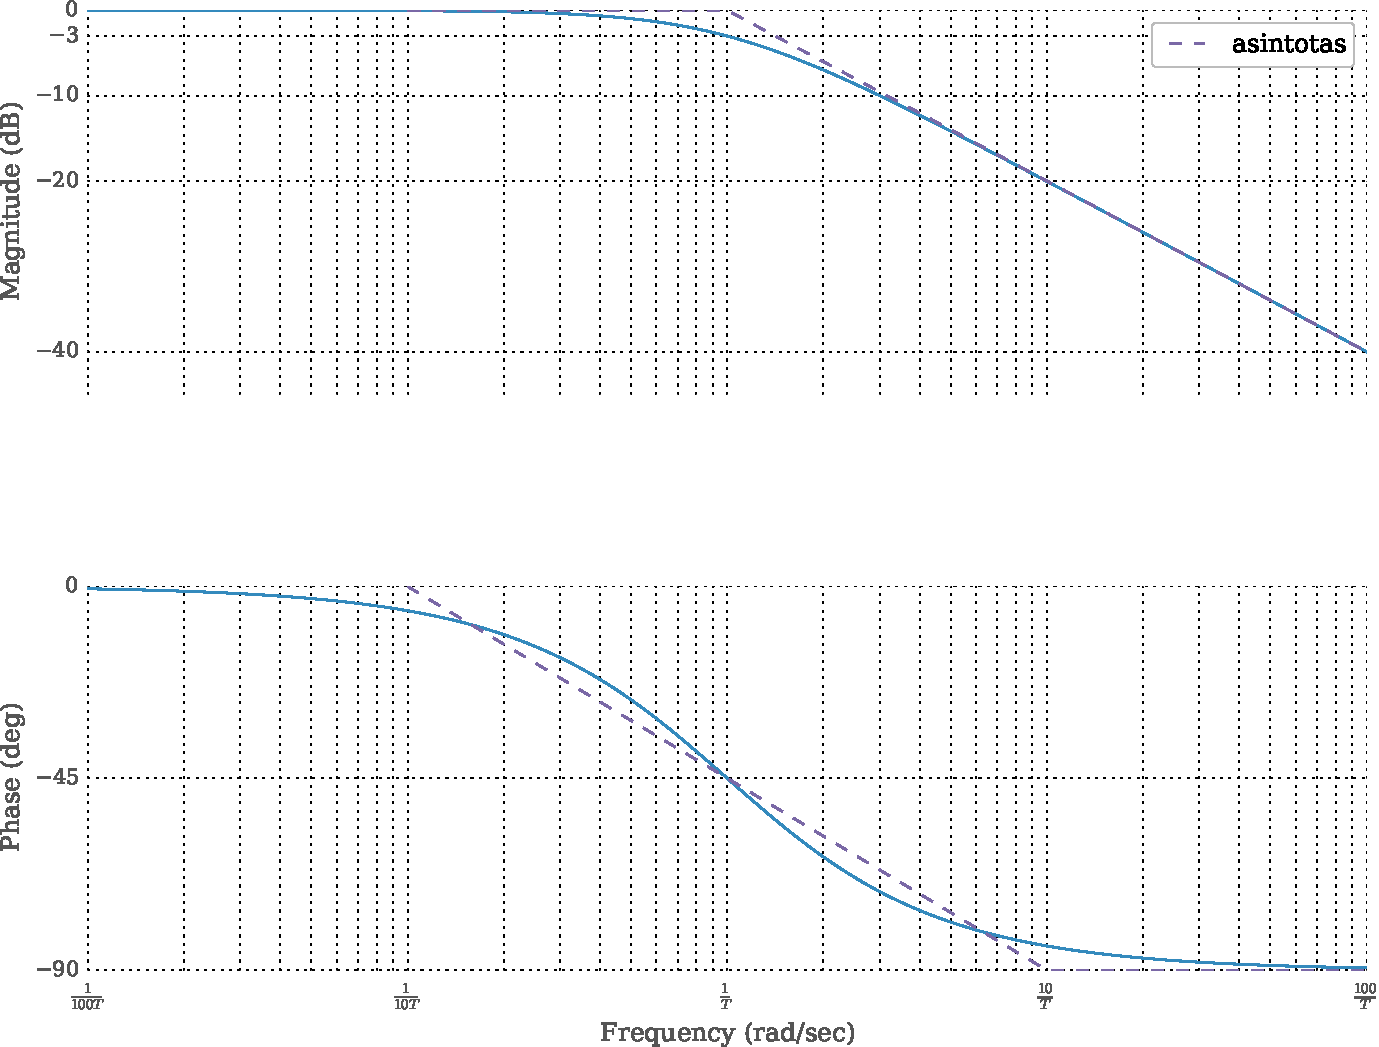
\includegraphics[width=\textwidth]{./imagenes/bodeprimerorden.pdf}
            \caption{\label{fig:bodeprimerorden}Diagrama de Bode del sistema $G(s) = \frac{1}{Ts + 1}$.}
        \end{marginfigure}

        De manera similar podemos gráficar el sistema inverso $G(s) =Ts + 1$ en la figura~\ref{fig:bodeprimerordeninverso}.

        \begin{marginfigure}
            \centering
            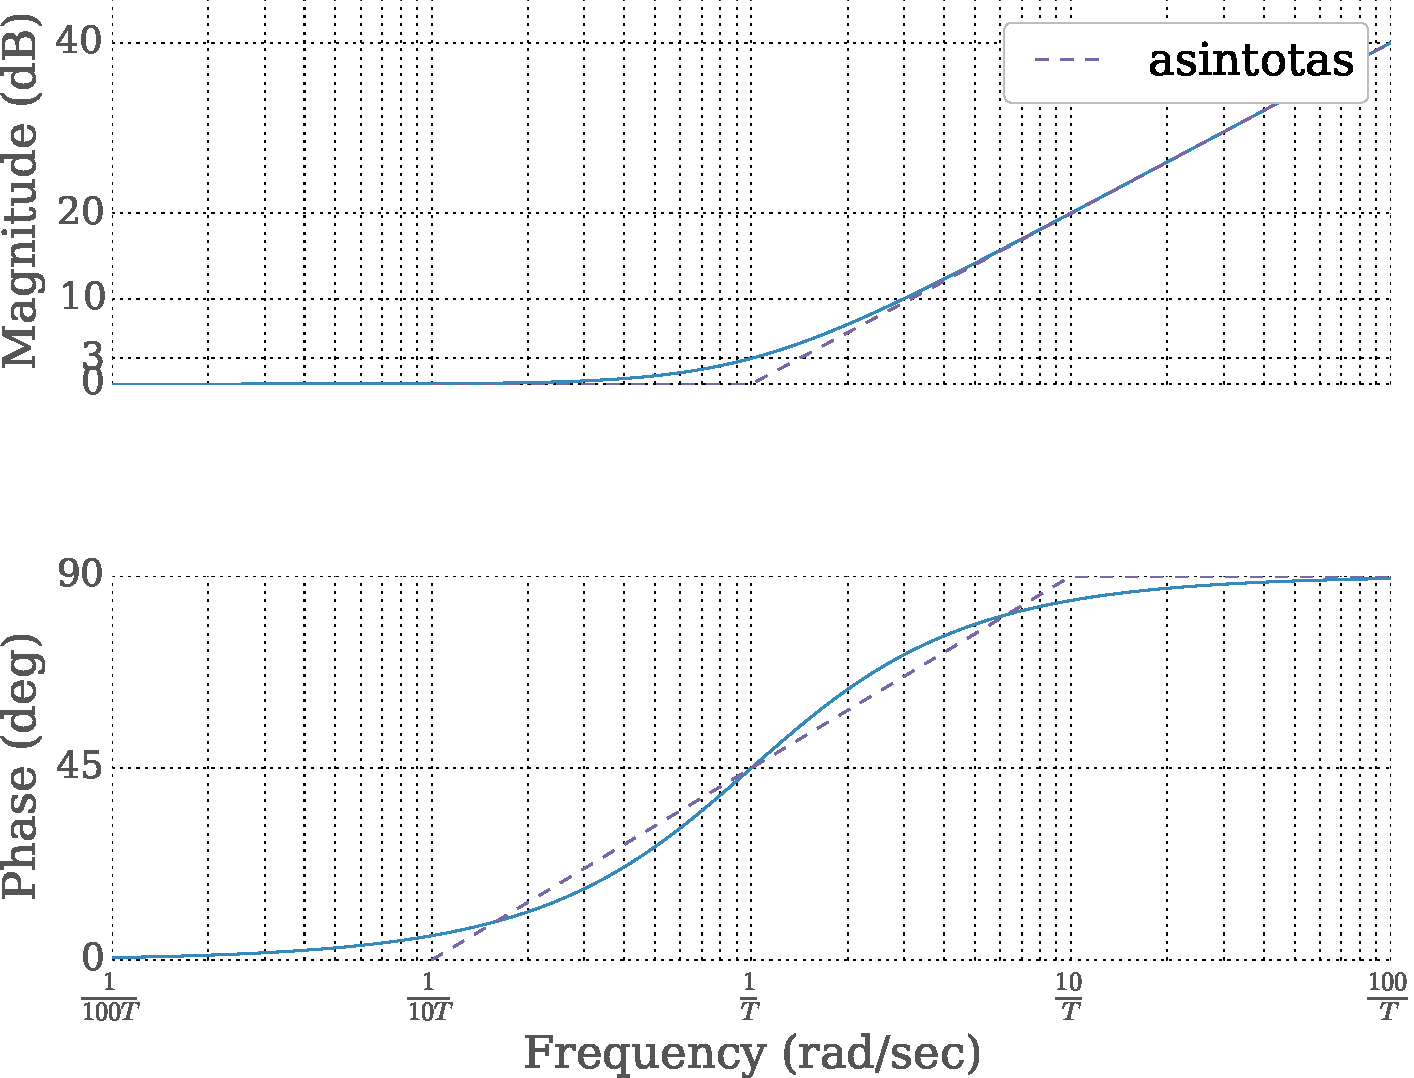
\includegraphics[width=\textwidth]{./imagenes/bodeprimerordeninverso.pdf}
            \caption{\label{fig:bodeprimerordeninverso}Diagrama de Bode del sistema $G(s) = Ts + 1$.}
        \end{marginfigure}

%-------------------------------------------------------------------------------
%	EMPIEZA SECCION
%-------------------------------------------------------------------------------

        \newpage
        \section{Factor integral}

            Dado el sistema $G(s) = \frac{1}{s}$ tendremos los siguientes valores para la magnitud y la fase:

            \begin{eqnarray*}
                \left| G(j \omega) \right|_{dB} & = & \left| \frac{1}{j \omega} \right|_{dB} = -20 \log{(\omega)} \\
                \phase{G(j \omega)} & = & -90^o
            \end{eqnarray*}

            Por lo que el diagrama de Bode queda como en la figura~\ref{fig:bodeintegral}.

            \begin{marginfigure}
                \centering
                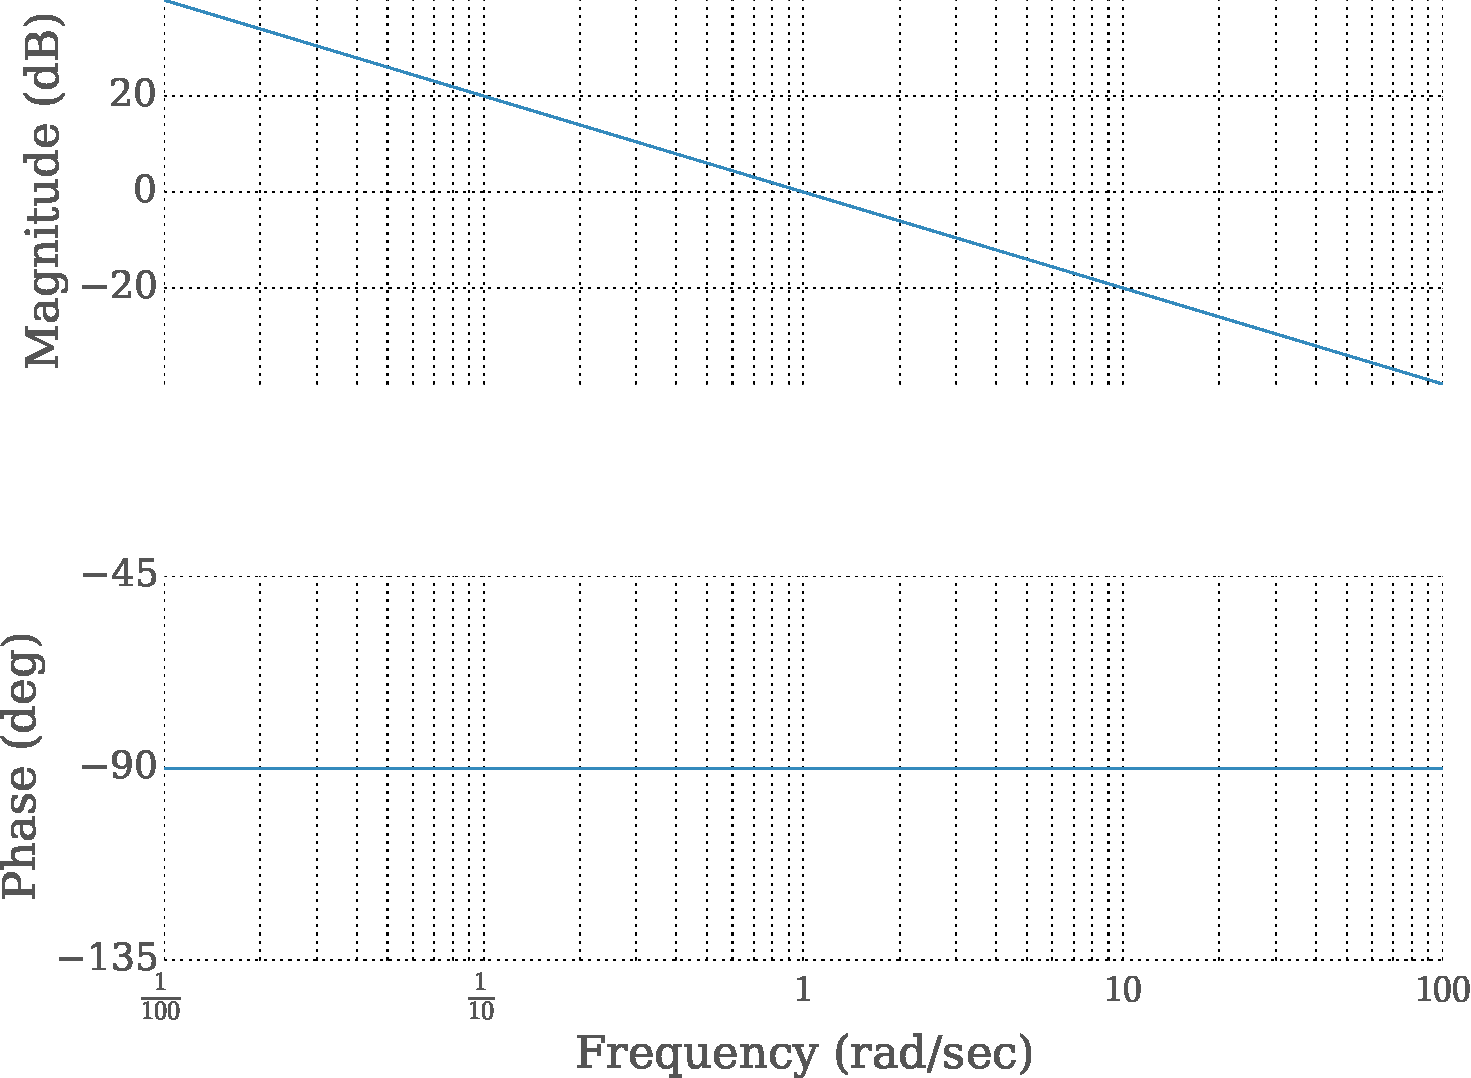
\includegraphics[width=\textwidth]{./imagenes/bodeintegral.pdf}
                \caption{\label{fig:bodeintegral}Diagrama de Bode del sistema $G(s) = \frac{1}{s}$.}
            \end{marginfigure}

%-------------------------------------------------------------------------------
%	EMPIEZA SECCION
%-------------------------------------------------------------------------------

        \newpage
        \section{Factor derivativo}

            Dado el sistema $G(s) = s$ tendremos los siguientes valores para la magnitud y la fase:

            \begin{eqnarray*}
                \left| G(j \omega) \right|_{dB} & = & \left| j \omega \right|_{dB} = 20 \log{(\omega)} \\
                \phase{G(j \omega)} & = & 90^o
            \end{eqnarray*}

            Por lo que el diagrama de Bode queda como en la figura~\ref{fig:bodederivativo}.

            \begin{marginfigure}
                \centering
                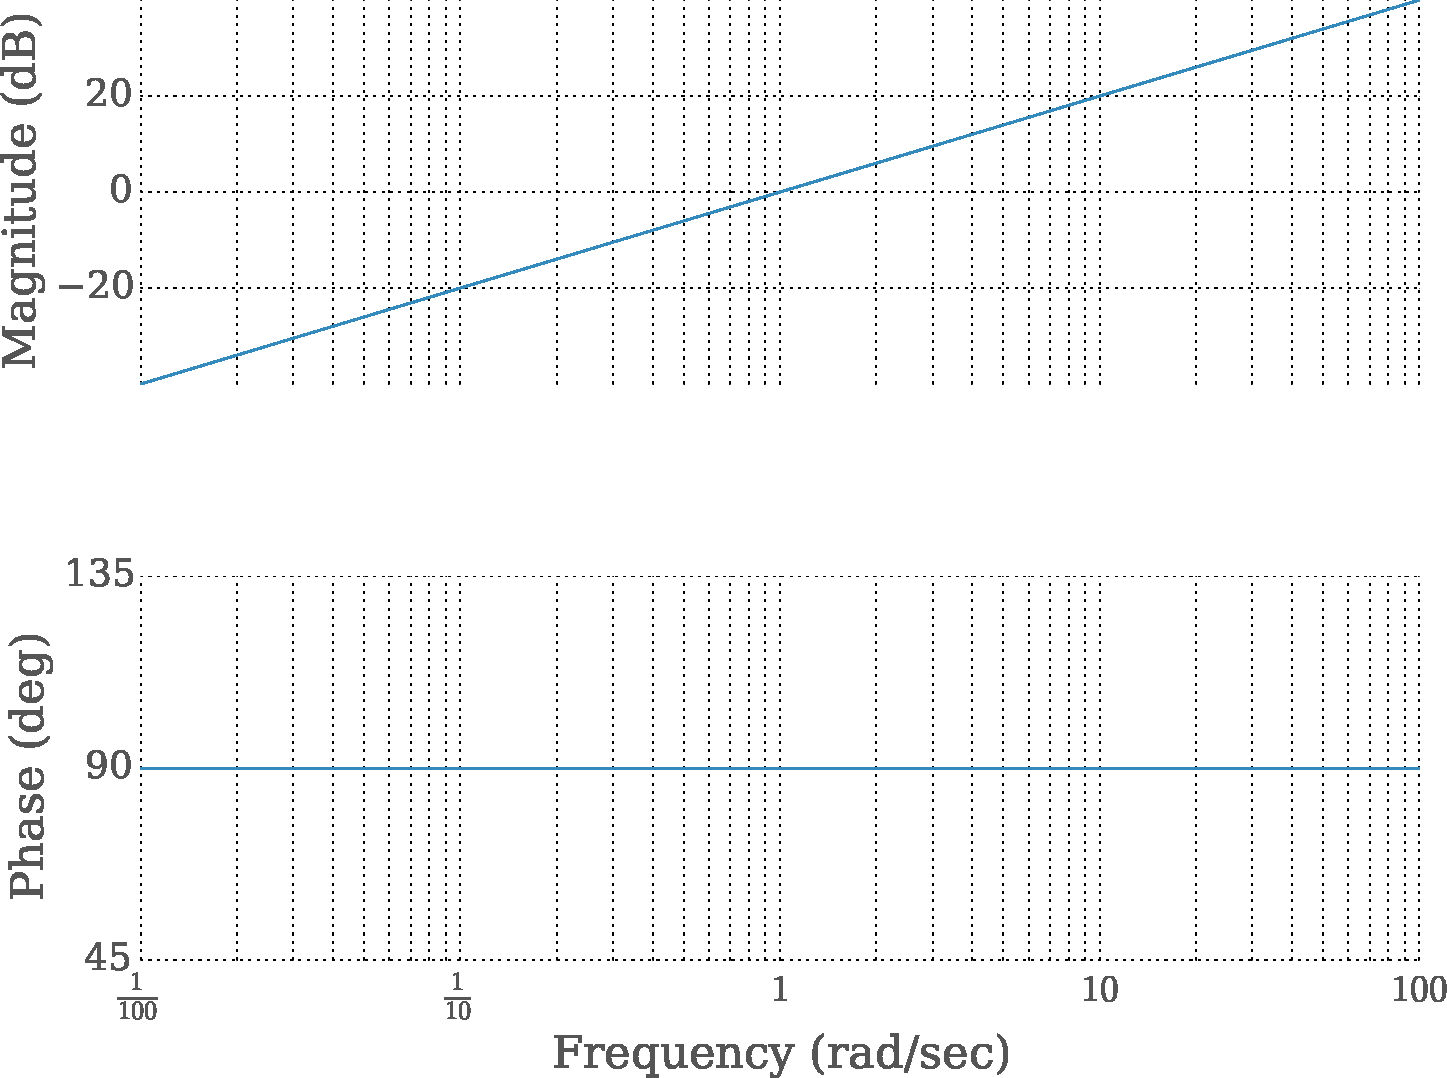
\includegraphics[width=\textwidth]{./imagenes/bodederivativo.pdf}
                \caption{\label{fig:bodederivativo}Diagrama de Bode del sistema $G(s) = s$.}
            \end{marginfigure}

%-------------------------------------------------------------------------------
%	EMPIEZA SECCION
%-------------------------------------------------------------------------------

    \newpage
    \section{Factores de segundo orden}

        Dado el sistema de segundo orden

        \begin{equation*}
            G(s) = \frac{1}{\left( \frac{s}{\omega_n} \right)^2 + 2 \zeta \left( \frac{s}{\omega_n} \right) + 1}
        \end{equation*}

        tendremos que su magnitud y fase estarán dados por:

        \begin{eqnarray*}
            \left| G(j \omega) \right|_{dB} & = & -20 \log{\sqrt{\left( 1 - \left( \frac{\omega}{\omega_n} \right)^2 \right)^2 + \left( 2 \zeta \left( \frac{\omega}{\omega_n} \right) \right)^2}} \\
            \phase{G(j \omega)} & = & -\arctan{\left( \frac{2 \zeta \left( \frac{\omega}{\omega_n} \right)}{1 - \left( \frac{\omega}{\omega_n} \right)^2} \right)}
        \end{eqnarray*}

        De estas ecuaciones, podemos aproximar su comportamiento cuando $\frac{\omega}{\omega_n}$ es muy grande o muy pequeño:

        \begin{eqnarray*}
            \frac{\omega}{\omega_n} \ll 1 & \implies & \left| G(j \omega) \right|_{dB} \approx -20 \log{\sqrt{1}} = 0 dB \\
            \frac{\omega}{\omega_n} \gg 1 & \implies & \left| G(j \omega) \right|_{dB} \approx -20 \log{\sqrt{\left( \frac{\omega}{\omega_n} \right)^4}} = -40 \log{\left( \frac{\omega}{\omega_n} \right)} dB
        \end{eqnarray*}

%-------------------------------------------------------------------------------

        \subsection{Frecuencia de resonancia $\omega_r$}

            Para encontrar la frecuencia de resonancia, necesitamos encontrar el punto en que la gráfica de magnitud cambia de dirección, es decir cuando la derivada cambia de signo. Por comodidad lo haremos con la función auxiliar $g(s) = \left( 1 - \left( \frac{\omega}{\omega_n} \right)^2 + \left( 2 \zeta \left( \frac{\omega}{\omega_n} \right) \right)^2 \right)$. Asi pues, la derivada será:

            \begin{eqnarray*}
                \frac{d g}{d \omega} & = & 2 \left( 1 - \left( \frac{\omega}{\omega_n} \right)^2 \right) \left( -2 \frac{\omega}{\omega_n} \right) + 4 \zeta^2 (2) \left( \frac{\omega}{\omega_n} \right) \\
                & = & -4 \frac{\omega}{\omega_n} \left( 1 - \left( \frac{\omega}{\omega_n} \right)^2 \right) + 4 \frac{\omega}{\omega_n} \left( 2 \zeta^2 \right) \\
                & = & 4 \frac{\omega}{\omega_n} \left( \left( \frac{\omega}{\omega_n} \right)^2 - 1 + 2 \zeta^2 \right) = 0
            \end{eqnarray*}

            por lo que la gráfica tiene pendiente nula cuando $\omega = 0$ o bien cuando $\left( \frac{\omega}{\omega_n} \right)^2 - 1 + 2 \zeta^2 = 0$, por lo que podemos ver que la frecuencia de resonancia se encuentra cuando:

            \begin{eqnarray*}
                \left( \frac{\omega}{\omega_n} \right)^2 & = & 1 - 2 \zeta^2 \\
                \frac{\omega}{\omega_n} & = & \sqrt{1 - 2 \zeta^2} \\
                \omega_r & = & \omega_n \sqrt{1 - 2 \zeta^2}
            \end{eqnarray*}

            donde $0 \le \zeta \le \frac{1}{\sqrt{2}}$.

%-------------------------------------------------------------------------------

        \subsection{Valor pico de resonancia $M_r$}

            Si sustituimos esta frecuencia de resonancia en la magnitud, tendremos el valor pico de resonancia.

            \begin{eqnarray*}
                M_r = \left| G(j \omega_r) \right|_{dB} & = & \frac{1}{\sqrt{\left( 1 - \left( \frac{\omega_n \sqrt{1 - 2 \zeta^2}}{\omega_n} \right)^2 + \left( 2 \zeta \left( \frac{\omega_n \sqrt{1 - 2 \zeta^2}}{\omega_n} \right) \right)^2 \right)}} \\
                & = & \frac{1}{\sqrt{\left( 1 - \left( \sqrt{1 - 2 \zeta^2} \right)^2 + \left( 2 \zeta \left( \sqrt{1 - 2 \zeta^2} \right) \right)^2 \right)}} \\
                & = & \frac{1}{\sqrt{4 \zeta^4 + 4 \zeta^2 \left( 1 - 2 \zeta^2 \right)}} \\
                & = & \frac{1}{2 \zeta \sqrt{\zeta^2 + 1 - 2 \zeta^2}} = \frac{1}{2 \zeta \sqrt{1 - \zeta^2}}
            \end{eqnarray*}

            Note que para diferentes valores de amortiguamiento tenemos:

            \begin{eqnarray*}
                \zeta = 0 & \implies & \omega_r = \omega_n \text{ y } M_r \to \infty \\
                \zeta = \frac{1}{\sqrt{2}} & \implies & \omega_r = 0 \text{ y } M_r = 1 \\
                \zeta > \frac{1}{\sqrt{2}} & \implies & M_r = 1
            \end{eqnarray*}

            Tendremos pues el diagrama de Bode de la figura~\ref{fig:bodesegundoorden}.

            \begin{marginfigure}
                \centering
                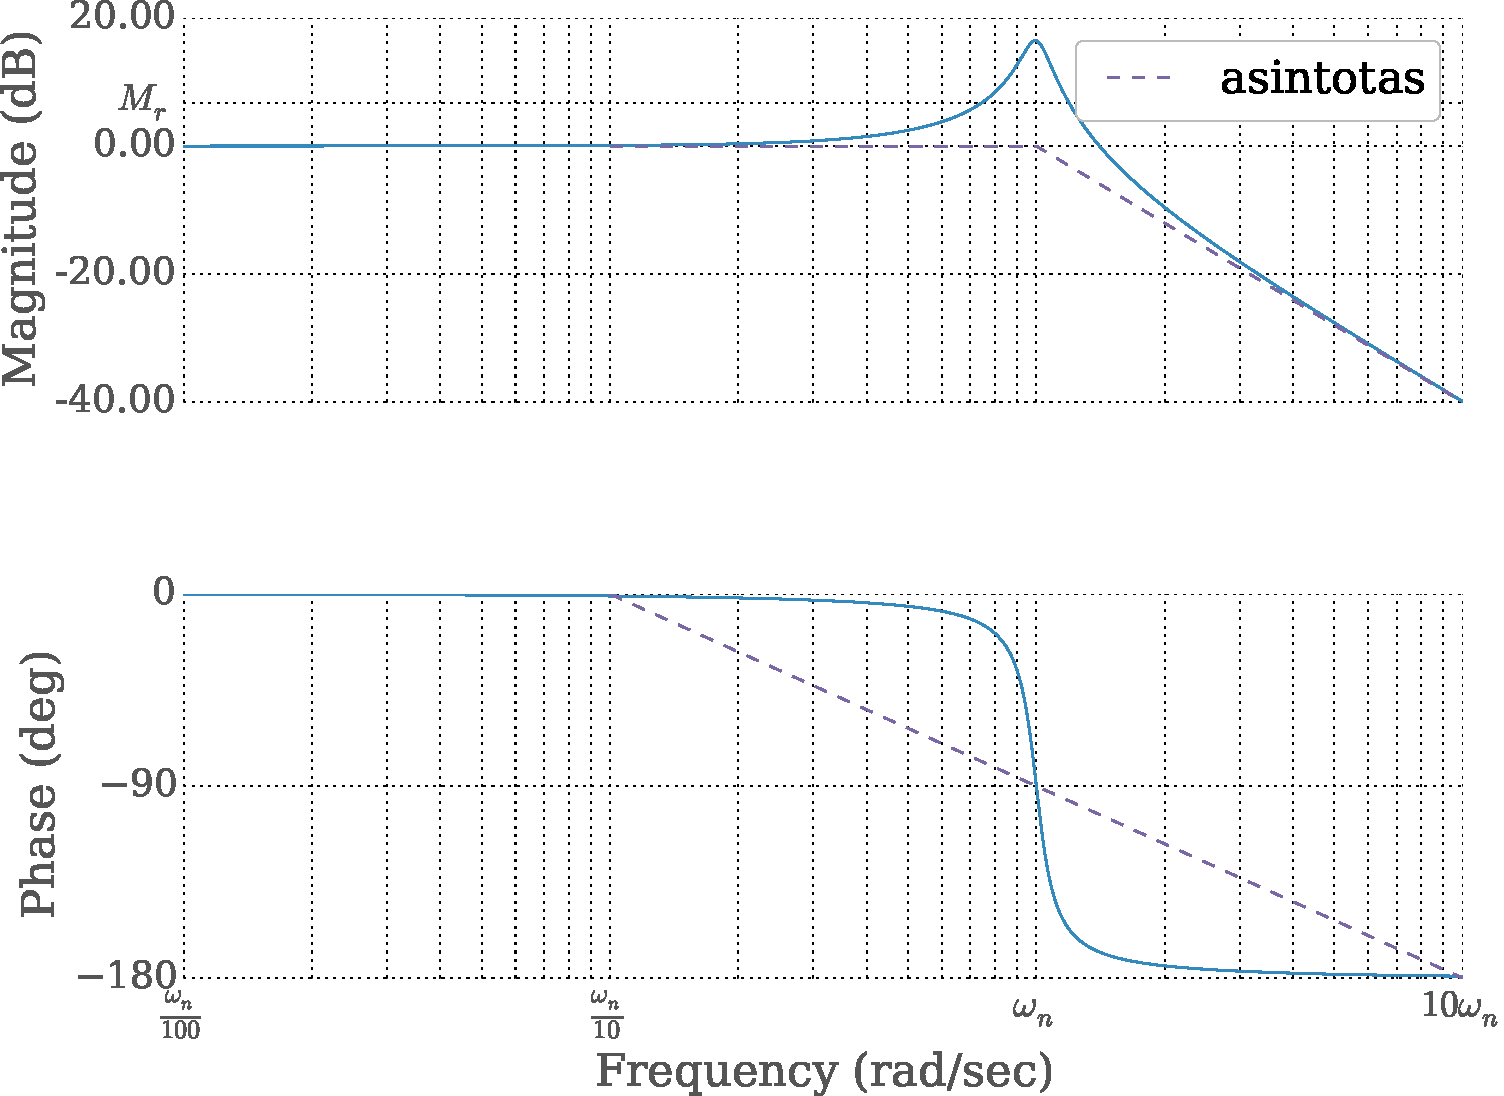
\includegraphics[width=\textwidth]{./imagenes/bodesegundoorden.pdf}
                \caption{\label{fig:bodesegundoorden}Diagrama de Bode del sistema $G(s) = \frac{1}{\left( \frac{s}{\omega_n} \right)^2 + 2 \zeta \left( \frac{s}{\omega_n} \right) + 1}$.}
            \end{marginfigure}

            y el inverso en la figura~\ref{fig:bodesegundoordeninverso}.

            \begin{marginfigure}
                \centering
                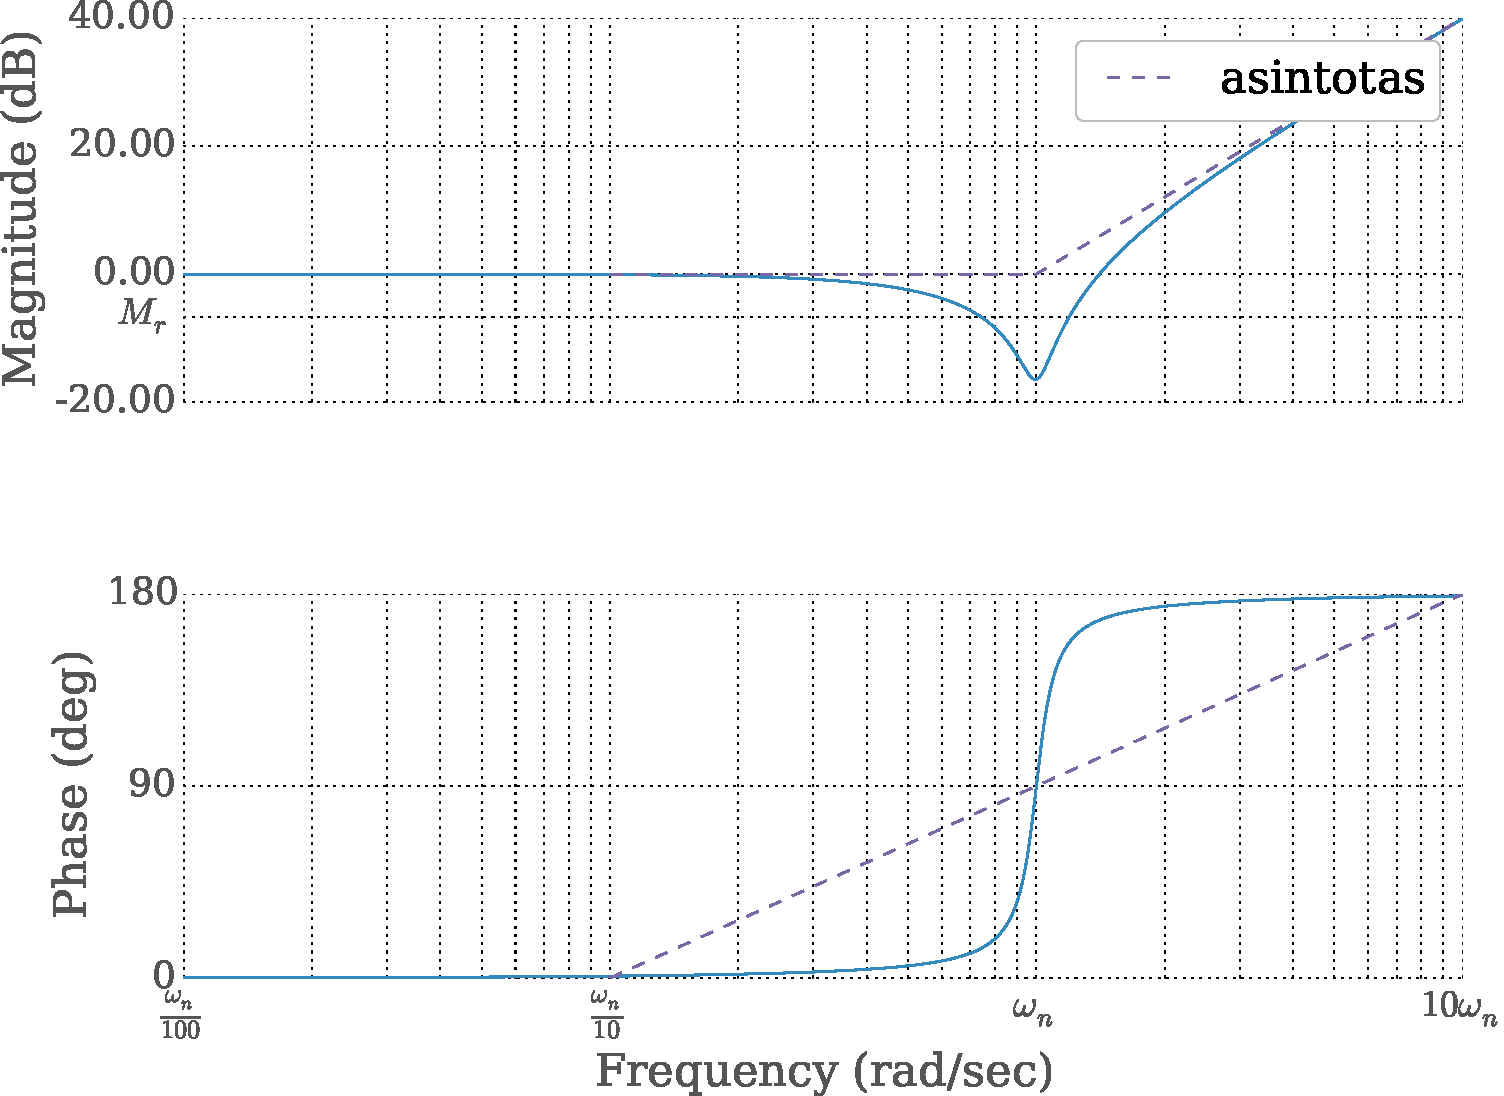
\includegraphics[width=\textwidth]{./imagenes/bodesegundoordeninverso.pdf}
                \caption{\label{fig:bodesegundoordeninverso}Diagrama de Bode del sistema $G(s) = \left( \frac{s}{\omega_n} \right)^2 + 2 \zeta \left( \frac{s}{\omega_n} \right) + 1$.}
            \end{marginfigure}

%-------------------------------------------------------------------------------
%	EMPIEZA SECCION
%-------------------------------------------------------------------------------

    \newpage
    \section{Factores de orden cero}
        Tan solo podemos notar rapidamente que los factores de orden cero, o ganancias, no tienen una dinámica asociada, por lo tanto sus diagramas de Bode son muy simples de graficar.

        \begin{equation*}
            G(s) = k
        \end{equation*}

        por lo que tendremos magnitud y fase:

        \begin{eqnarray*}
            \left| G(j \omega) \right|_{dB} & = & 20 \log{k} \\
            \phase{G(j \omega)} & = & 0^o
        \end{eqnarray*}

        y sus diagramas de bode, los de la figura~\ref{fig:bodeordencero}.

        \begin{marginfigure}
            \centering
            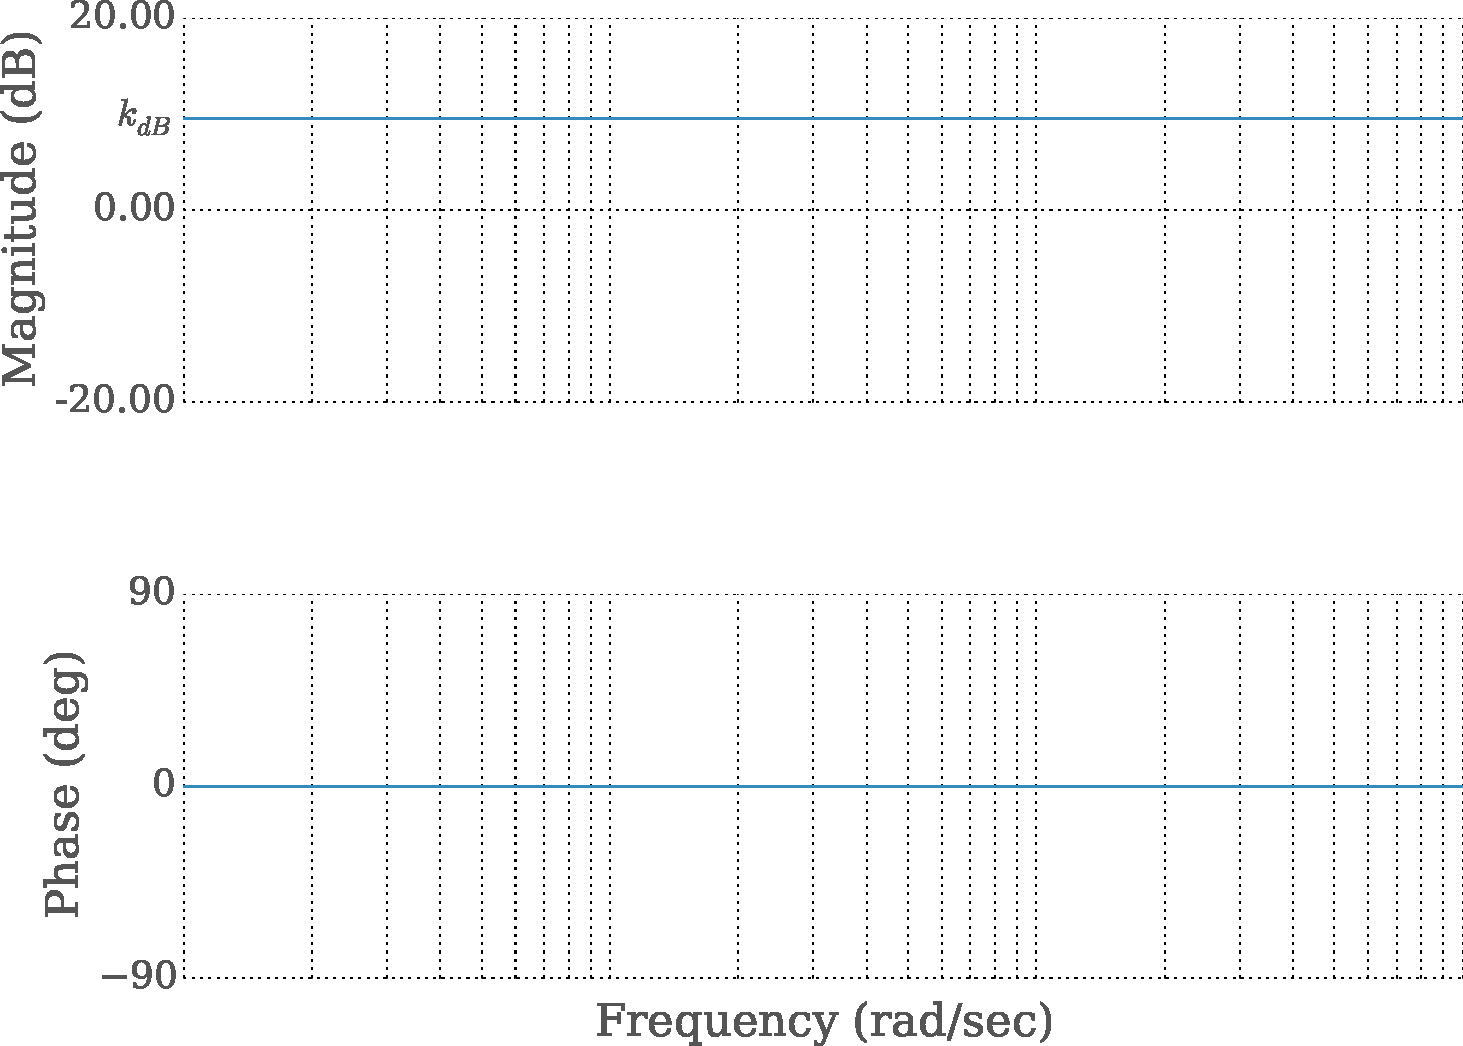
\includegraphics[width=\textwidth]{./imagenes/bodeordencero.pdf}
            \caption{\label{fig:bodeordencero}Diagrama de Bode del sistema $G(s) = k$.}
        \end{marginfigure}
